% This file was created by matplotlib2tikz v0.7.4.
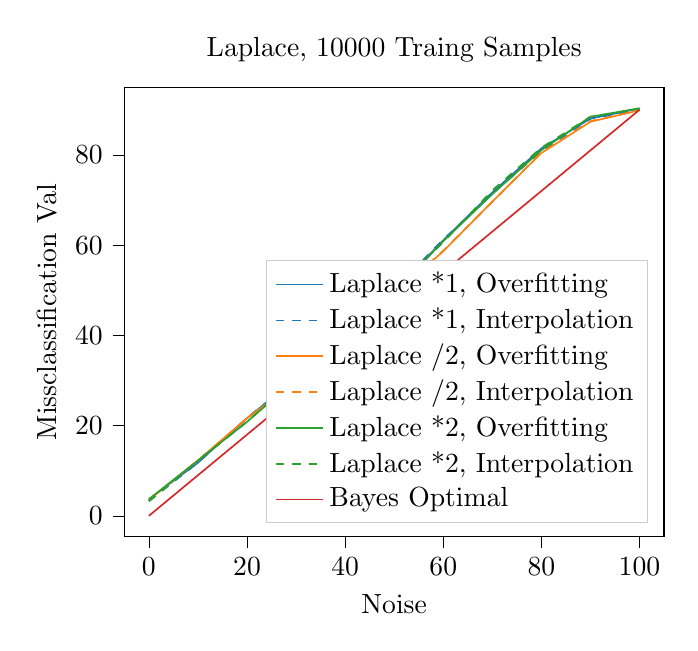
\begin{tikzpicture}

\definecolor{color0}{rgb}{0.12156862745098,0.466666666666667,0.705882352941177}
\definecolor{color1}{rgb}{1,0.498039215686275,0.0549019607843137}
\definecolor{color2}{rgb}{0.172549019607843,0.627450980392157,0.172549019607843}
\definecolor{color3}{rgb}{0.83921568627451,0.152941176470588,0.156862745098039}

\begin{axis}[
legend cell align={left},
legend style={at={(0.97,0.03)}, anchor=south east, draw=white!80.0!black},
tick align=outside,
tick pos=left,
title={Laplace, 10000 Traing Samples},
x grid style={white!69.01960784313725!black},
xlabel={Noise},
xmin=-5, xmax=105,
xtick style={color=black},
y grid style={white!69.01960784313725!black},
ylabel={Missclassification Val},
ymin=-4.517, ymax=94.857,
ytick style={color=black}
]
\addplot [semithick, color0]
table {%
0 3.68000000000001
10 11.78
20 21.63
30 30.46
40 39.79
50 49.76
60 61.08
70 71.69
80 81.45
90 88.05
100 90.3
};
\addlegendentry{Laplace *1, Overfitting}
\addplot [semithick, color0, dashed]
table {%
0 3.27
10 11.78
20 21.71
30 30.46
40 39.89
50 50.25
60 61.24
70 71.36
80 80.87
90 88.02
100 89.97
};
\addlegendentry{Laplace *1, Interpolation}
\addplot [semithick, color1]
table {%
0 3.52
10 12.29
20 21.65
30 29.65
40 38.82
50 49.17
60 58.63
70 69.65
80 80.41
90 87.35
100 89.89
};
\addlegendentry{Laplace /2, Overfitting}
\addplot [semithick, color1, dashed]
table {%
0 3.49
10 12.3
20 21.6
30 29.59
40 38.87
50 49.11
60 58.77
70 69.6
80 80.52
90 87.47
100 89.91
};
\addlegendentry{Laplace /2, Interpolation}
\addplot [semithick, color2]
table {%
0 3.69
10 12.27
20 20.83
30 30.3
40 40.65
50 49.53
60 60.89
70 71.31
80 81.05
90 88.45
100 90.34
};
\addlegendentry{Laplace *2, Overfitting}
\addplot [semithick, color2, dashed]
table {%
0 3.19
10 12.19
20 20.87
30 30.4
40 40.84
50 50.18
60 60.64
70 72.15
80 81.6
90 88.47
100 90.2
};
\addlegendentry{Laplace *2, Interpolation}
\addplot [semithick, color3]
table {%
0 0
10 9
20 18
30 27
40 36
50 45
60 54
70 63
80 72
90 81
100 90
};
\addlegendentry{Bayes Optimal}
\end{axis}

\end{tikzpicture}